\documentclass[11pt,a4paper]{article}
\usepackage[utf8]{inputenc}
\usepackage[T1]{fontenc}
\usepackage{tgpagella}
\usepackage[spanish]{babel}
\usepackage{geometry}
\usepackage{booktabs}
\usepackage{xcolor}
\usepackage{titlesec}
\usepackage{fancyhdr}
\usepackage[parfill]{parskip}
\usepackage[expansion=false]{microtype}
\usepackage{hyperref}
\usepackage{setspace}
\usepackage{graphicx}
\usepackage{needspace}
\widowpenalty=10000
\clubpenalty=10000
\displaywidowpenalty=10000

\geometry{top=3.0cm,bottom=3.0cm,left=3.5cm,right=3.5cm}
\setlength{\parskip}{0.65em}
\setlength{\parindent}{0em}

\definecolor{azulai}{RGB}{30,80,140}
\definecolor{doradoai}{RGB}{140,90,0}
\definecolor{grisai}{RGB}{70,70,70}

\titleformat{\section}{\Large\bfseries\color{azulai}}{}{0em}{}[{\color{azulai}\titlerule[0.5pt]}]
\titlespacing*{\section}{0pt}{1.4em}{0.5em}

\titleformat{\subsection}{\large\bfseries\color{doradoai}}{}{0em}{}
\titlespacing*{\subsection}{0pt}{1.0em}{0.35em}

\titleformat{\subsubsection}{\normalsize\bfseries\color{grisai}}{}{0em}{}
\titlespacing*{\subsubsection}{0pt}{0.7em}{0.25em}

\pagestyle{fancy}\fancyhf{}
\rhead{\textcolor{grisai}{\small Amaya Beatriz — Arquitectura Interna}}
\lhead{\textcolor{grisai}{\small Urano · Neptuno · Plutón}}
\cfoot{\textcolor{grisai}{\small\thepage}}
\renewcommand{\headrulewidth}{0.3pt}

\hypersetup{colorlinks=true,linkcolor=azulai,urlcolor=azulai}
\setstretch{1.25}
\tolerance=1500
\emergencystretch=4em

\begin{document}

% ── Portada ──────────────────────────────────────────────────────────────────
\begin{titlepage}
  \centering
  \vspace*{1.5cm}
  {\Huge\bfseries\color{azulai} Urano · Neptuno · Plutón}\\[0.5cm]
  {\large\color{grisai} Arquitectura Interna}\\[0.3cm]
  {\small\itshape\color{grisai} Procesos profundos de cambio, sensibilidad y transformación}\[2cm]
  {\huge\color{doradoai} Amaya Beatriz}\\[1.5cm]
  {\Large 30/10/1976 \quad 22:10}\\[0.3cm]
  {\Large Zaragoza, España}\\[0.3cm]
  {\normalsize Lat: 41.6916° \quad Lon: -0.9101° \quad UTC+01:00}\\[0.3cm]
  {\normalsize Ascendente: Cáncer 16°08' \quad
    MC: Piscis 25°32'}\\[2cm]
  \begin{tabular}{ll}
    \textbf{Urano:}   & Escorpio — Casa 5 7°29'  \\
    \textbf{Neptuno:} & Sagitario — Casa 6 12°24' \\
    \textbf{Plutón:}  & Libra — Casa 4 12°36' \\
  \end{tabular}\\[2cm]
  \vfill
  {\small Generado el 19/05/2026}
\end{titlepage}

\tableofcontents
\newpage

% ── Datos de referencia ───────────────────────────────────────────────────────
\section{Datos de referencia}

\begin{center}
\begin{tabular}{llll}
  \toprule
  \textbf{Planeta} & \textbf{Signo} & \textbf{Casa} & \textbf{Posición} \\
  \midrule
  Urano    & Escorpio   & 5   & 7°29'  \\
  Neptuno & Sagitario  & 6  & 12°24' \\
  Plutón  & Libra  & 4  & 12°36' \\
  Sol              & Escorpio  & 5  & 7°35' \\
  Luna             & Acuario & 8 & 19°05' \\
  Ascendente       & Cáncer          & ---                   & 16°08' \\
  Medio Cielo      & Piscis           & ---                   & 25°32' \\
  \bottomrule
\end{tabular}
\end{center}

\vspace{0.5cm}
\textbf{Aspectos relevantes:}

\begin{center}
\begin{tabular}{lllll}
  \toprule
  \textbf{Planeta 1} & \textbf{Asp.} & \textbf{Planeta 2} & \textbf{Tipo} & \textbf{Orbe} \\
  \midrule
  Neptuno & conj & Venus & Conjunción & 0.0° \\
  Urano & conj & Sol & Conjunción & 0.1° \\
  Neptuno & sex & Plutón & Sextil & 0.2° \\
  Plutón & sex & Venus & Sextil & 0.2° \\
  Lilith & opo & Urano & Oposición & 3.1° \\
  Plutón & sex & Saturno & Sextil & 3.6° \\
  Neptuno & tri & Saturno & Trígono & 3.8° \\
  Urano & conj & Mercurio & Conjunción & 4.7° \\
  Plutón & tri & Luna & Trígono & 6.5° \\
  Urano & conj & Marte & Conjunción & 7.6° \\
  Quirón & opo & Urano & Oposición & 7.8° \\
  \bottomrule
\end{tabular}
\end{center}

\begin{center}
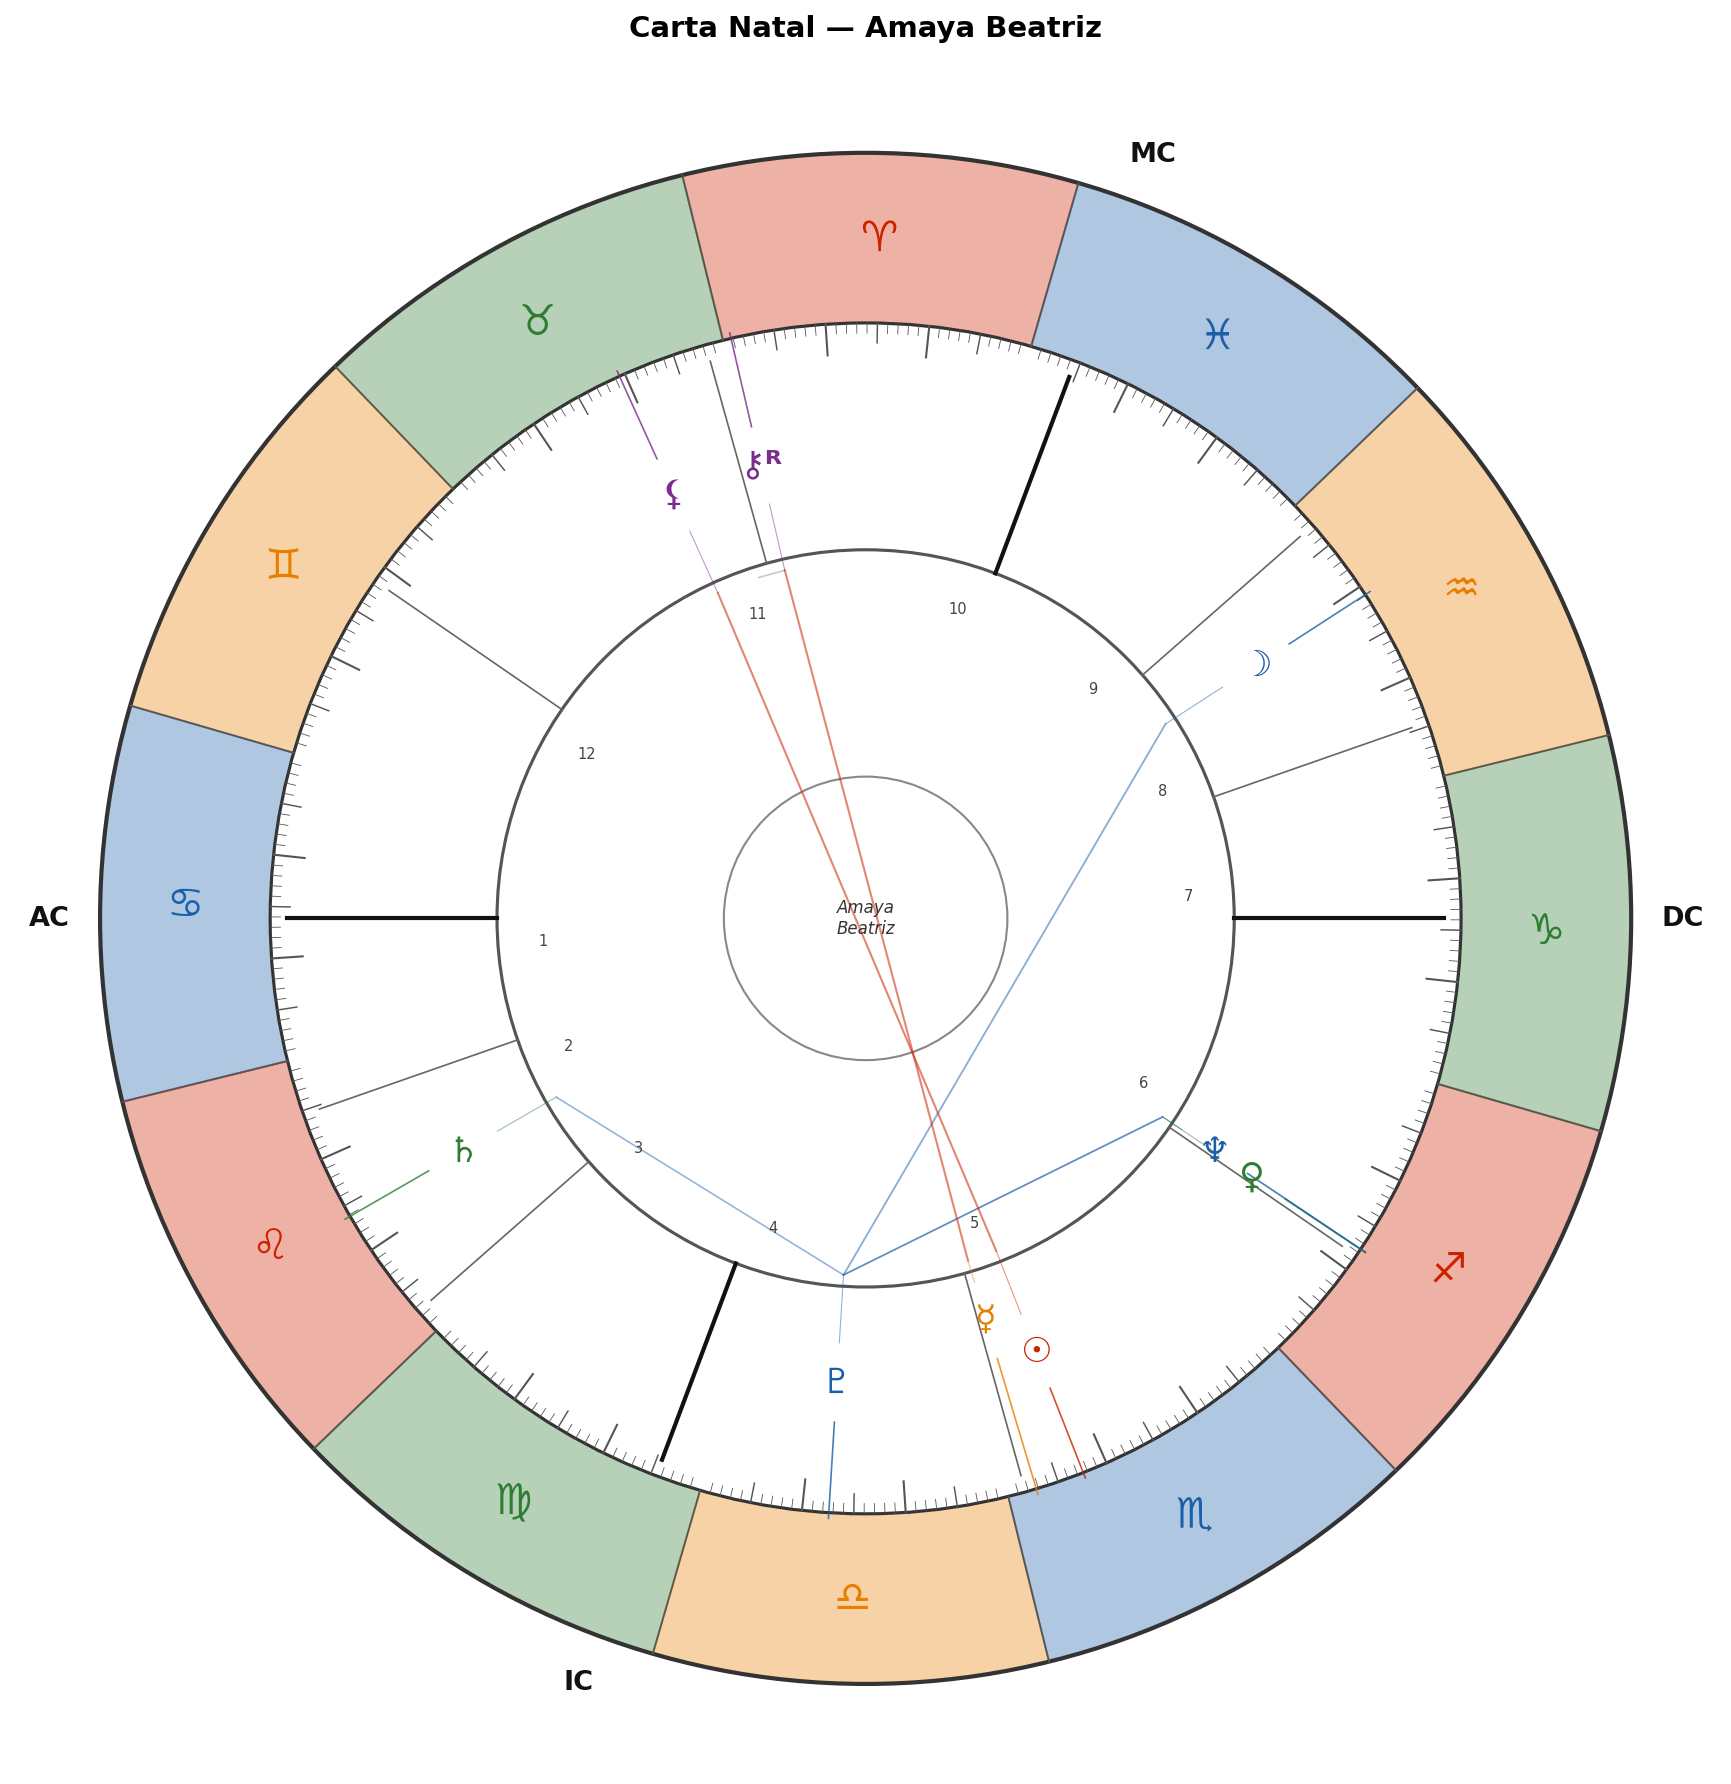
\includegraphics[width=0.72\textwidth]{Amaya_Beatriz_rueda.png}
\end{center}

\Needspace{3\baselineskip}


% ── Interpretación ────────────────────────────────────────────────────────────
\section{Interpretación — Arquitectura Interna}

\begin{center}
{\small\itshape
No se trata de describir la personalidad. Se trata de mostrar qué procesos\\
de cambio, sensibilidad y transformación pueden activarse en tu vida.
}
\end{center}

\vspace{0.8cm}
\Needspace{5\baselineskip}

% ── 1. Marco general ──────────────────────────────────────────────────────────
\subsection{1. Marco general}

Urano, Neptuno y Plutón no describen lo más cotidiano o visible de tu carta. Muestran procesos más profundos, menos controlables, que pueden modificar tu forma de vivir, sostenerte y atravesar determinadas etapas.

Urano en Escorpio, Casa 5: muestra dónde aparecen cambios, interrupciones o necesidad de libertad. Cuando se activa, algo que antes funcionaba puede dejar de hacerlo igual.
Neptuno en Sagitario, Casa 6: muestra dónde los límites se vuelven más sensibles, difusos o permeables. Cuando se activa, algo que parecía claro puede perder forma.
Plutón en Libra, Casa 4: muestra dónde aparecen procesos intensos de transformación. Cuando se activa, algo que se sostenía de una manera ya no puede seguir igual.

Aspectos activos con planetas personales: Urano–Sol en conjunción (orbe 0.09°), Urano–Mercurio en conjunción (orbe 4.69°), Urano–Marte en conjunción (orbe 7.63°), Neptuno–Venus en conjunción (orbe 0.04°), Plutón–Luna en trígono (orbe 6.49°), Plutón–Venus en sextil (orbe 0.23°).

\vspace{0.8cm}
\Needspace{5\baselineskip}


% ── 2. Urano ──────────────────────────────────────────────────────────────────
\subsection{2. Urano — Ruptura y cambio de patrón}

\subsubsection*{Urano en Escorpio — Casa 5}

Urano en Escorpio muestra cambios intensos y difíciles de controlar en procesos emocionales profundos. Hay una necesidad constante de transformación, incluso cuando una parte de ti preferiría mantener el control.

Puede haber rupturas internas importantes, descubrimientos difíciles de ignorar o momentos donde algo cambia de forma irreversible. A veces lo que intentabas contener termina emergiendo de golpe.

El aprendizaje está en permitir transformación sin vivir cada cambio como una amenaza que necesitas controlar completamente.

Urano en Casa 5 muestra necesidad de expresarte de forma libre, auténtica y poco convencional. Puede costarte sostener formas creativas demasiado previsibles o repetitivas.

A veces aparecen etapas de mucha inspiración seguidas de cortes bruscos o cambios de dirección. También puede haber giros importantes en la forma de vivir el deseo, la creatividad o la necesidad de reconocimiento.

El aprendizaje está en sostener la creatividad sin necesitar romper constantemente con lo que estabas construyendo.

Urano en conjunción con el Sol hace que los cambios afecten directamente a tu dirección de vida y a la forma en que necesitas afirmarte. Es difícil sostener durante mucho tiempo caminos, decisiones o identidades que ya no sientes vivas.

Puede haber necesidad constante de cambio, etapas de giros importantes o dificultad para mantener una dirección estable durante largos periodos.

El aprendizaje está en permitir evolución sin sentir que necesitas romperlo todo cada vez que algo cambia.

Urano en conjunción con Mercurio hace que la mente funcione de forma rápida, intuitiva y poco lineal. Las ideas aparecen de golpe y muchas veces necesitas cambiar de perspectiva constantemente.

Puede haber mucha creatividad mental, asociaciones inesperadas o dificultad para sostener formas de pensamiento demasiado rígidas.

El aprendizaje pasa por ordenar las ideas sin perder frescura ni capacidad de innovación.

Urano en conjunción con Marte intensifica muchísimo la necesidad de actuar con libertad y rapidez. Puede costarte contener impulsos o sostener durante mucho tiempo acciones demasiado lentas o limitantes.

A veces actúas de forma repentina, cambias de dirección rápidamente o necesitas movimiento constante para sentir vitalidad.

El aprendizaje está en canalizar la energía sin vivir permanentemente desde la impulsividad o la ruptura.

\vspace{0.8cm}
\Needspace{5\baselineskip}

% ── 3. Neptuno ────────────────────────────────────────────────────────────────
\subsection{3. Neptuno — Disolución y pérdida de forma}

\subsubsection*{Neptuno en Sagitario — Casa 6}

Neptuno en Sagitario puede hacer que busques sentido, dirección o verdad en lugares que después resultan menos sólidos de lo que parecían. A veces necesitas creer en algo para sentir orientación, incluso cuando todavía no está claro.

Puede haber idealización de caminos, proyectos, filosofías o personas que parecen ofrecer amplitud o propósito. También puedes cambiar varias veces de dirección buscando una referencia más auténtica.

El aprendizaje está en desarrollar una visión más consciente sin perder apertura ni capacidad de inspiración.

Neptuno en Casa 6 vuelve más difusos los límites relacionados con trabajo, hábitos y funcionamiento cotidiano. Puede costarte mantener rutinas claras o reconocer a tiempo cuándo algo te está agotando.

A veces hay confusión en horarios, organización o formas de cuidar el cuerpo y la energía. También puedes absorber demasiado del ambiente laboral o de las exigencias externas.

El aprendizaje está en desarrollar hábitos más conscientes y sostenibles sin rigidizarte.

Neptuno en conjunción con Venus intensifica muchísimo la sensibilidad afectiva y la tendencia a idealizar vínculos o experiencias emocionales. Puede costarte ver con claridad qué ocurre realmente en una relación.

A veces hay mucha entrega, romanticismo o necesidad de conexión profunda, pero también dificultad para sostener límites claros.

El aprendizaje está en amar sin perder completamente la referencia de ti.

\vspace{0.8cm}
\Needspace{5\baselineskip}

% ── 4. Plutón ─────────────────────────────────────────────────────────────────
\subsection{4. Plutón — Intensidad y transformación profunda}

\subsubsection*{Plutón en Libra — Casa 4}

Plutón en Libra intensifica profundamente los vínculos y la necesidad de equilibrio real en las relaciones. Las transformaciones suelen aparecer a través de acuerdos, rupturas o dinámicas relacionales difíciles de sostener superficialmente.

Puede haber miedo a perder vínculos importantes, relaciones muy intensas o dificultad para mantener relaciones donde no existe reciprocidad verdadera.

El aprendizaje pasa por construir vínculos más honestos y profundos sin quedar atrapade en dinámicas de dependencia o control.

Plutón en Casa 4 intensifica muchísimo la vida emocional profunda, la historia familiar y la sensación de base interna. Las transformaciones suelen afectar directamente a lo que sentías como refugio o estabilidad emocional.

Puede haber necesidad de revisar patrones muy antiguos, emociones profundas o formas de protección que ya no funcionan igual.

El aprendizaje pasa por construir una base más consciente sin intentar mantener intacto lo que necesita transformarse.

Plutón en trígono a la Luna facilita integrar profundidad emocional y capacidad de transformación interna. Las emociones intensas suelen ayudarte a crecer y comprenderte mejor.

Existe capacidad para atravesar procesos emocionales profundos sin perder completamente estabilidad interna.

El aprendizaje pasa por utilizar esa profundidad emocional de forma consciente y constructiva.

Plutón en sextil a Venus facilita transformar vínculos y patrones afectivos de manera bastante consciente. Existe capacidad para reconocer antes qué relaciones o dinámicas necesitan cambiar.

Las experiencias emocionales profundas suelen ayudarte a comprender mejor qué valoras realmente.

El aprendizaje está en permitir transformación afectiva sin esperar siempre a llegar al límite.

\vspace{0.8cm}
\Needspace{5\baselineskip}

% ── 5. Integración ────────────────────────────────────────────────────────────
\subsection{5. Integración — Las tres fuerzas en tu carta}

Urano, Neptuno y Plutón actúan de formas distintas y no siempre coordinadas. Urano en Escorpio, Casa 5, muestra dónde aparecen cambios, interrupciones o necesidad de libertad. Cuando se activa, algo que antes funcionaba puede dejar de hacerlo igual. Neptuno en Sagitario, Casa 6, muestra dónde los límites se vuelven más sensibles, difusos o difíciles de sostener. Cuando se activa, algo que parecía claro puede perder forma. Plutón en Libra, Casa 4, muestra dónde aparecen procesos intensos de transformación. Cuando se activa, algo que sostenías de una manera ya no puede seguir igual.

Neptuno en Sagitario muestra una sensibilidad especial en ciertas áreas de tu vida: tiendes a desbordarte por exceso de impulso o dificultad para frenar a tiempo. Urano en Escorpio muestra cómo suelen producirse los cambios importantes: los cambios aparecen cuando cambia lo que sientes profundamente. Plutón en Libra concentra la intensidad en procesos que no pueden quedarse igual indefinidamente: determinadas experiencias terminan empujándote a transformar algo en profundidad.

En determinados momentos, estas tres fuerzas pueden activarse de forma encadenada. Urano en Escorpio suele aparecer primero: cambian vínculos, emociones o sensaciones de pertenencia de forma repentina. Después, Neptuno en Sagitario puede hacer que aparezca sensación de confusión, pérdida de claridad o dificultad para entender bien qué está pasando: la energía pierde dirección y cuesta saber hacia dónde moverte. Finalmente, Plutón en Libra concentra la intensidad en aquello que ya no puede seguir igual: la intensidad se concentra en pensamientos, conversaciones o formas de comprender la vida. Por eso, determinadas etapas pueden sentirse especialmente intensas: no estás viviendo una sola cosa, sino varios procesos moviéndose al mismo tiempo.

\vspace{0.8cm}
\Needspace{5\baselineskip}

% ── 6. Orientación ────────────────────────────────────────────────────────────
\subsection{6. Orientación}

\subsubsection*{Cuando Urano está activo}
Urano suele activarse cuando: aparecen cambios emocionales o relacionales difíciles de prever. Esto suele sentirse especialmente en temas relacionados con la Casa 5.

\subsubsection*{Cuando Neptuno está activo}
Neptuno suele activarse cuando: pierdes claridad sobre hacia dónde quieres dirigirte. Esto suele sentirse especialmente en temas relacionados con la Casa 6.

\subsubsection*{Cuando Plutón está activo}
Plutón suele activarse cuando: determinados pensamientos o conversaciones adquieren mucha intensidad y profundidad. Esto suele sentirse especialmente en temas relacionados con la Casa 4.

\subsubsection*{Cuando no se reconocen}
Cuando estos procesos no se reconocen, es fácil vivirlos únicamente como problemas externos o mala suerte. Sin embargo, muchas veces están mostrando que algo necesita cambiar, redefinirse o transformarse más profundamente.

Intentar sostener exactamente igual algo que internamente ya está cambiando suele generar más desgaste, más confusión o más sensación de bloqueo.

\vspace{0.6cm}
Si estos procesos se ignoran durante mucho tiempo, suelen intensificarse. Urano puede traer cambios cada vez más bruscos. Neptuno puede aumentar la sensación de confusión, desgaste o pérdida de claridad. Plutón puede concentrar tanta intensidad que determinadas situaciones ya no puedan seguir sosteniéndose igual.

Por eso, reconocer antes lo que está cambiando suele ayudar a atravesar estas etapas con más consciencia y menos ruptura.

\vspace{1cm}
\begin{center}
{\small\itshape\color{grisai}
La astrología se usa aquí como lenguaje simbólico de observación, no como definición de la persona.\
Este documento es una aproximación funcional, no un diagnóstico.
}
\end{center}

\end{document}
